\scanpage{28}
\mspage{14}
fundamental groups are \inserted{apparently} trivial :
\[
\pi_1(\mathcal T_{0\nu})=0\qquad 0\leq\nu\leq3
\]
The Topos $\mathcal T_{0,\nu}$ \deleted{is the \inserted{big} fibred topos} \inserted{$(\nu\geq4)$ corresponds to the} \deleted{étale of} \inserted{scheme} of systems of $\nu-3$ distinct points $(x_1,\begin{tikzpicture}[baseline=-.4ex,x=1em,y=1em,line cap=round]
\draw[line width=.35pt] (0,0) -- (.32,.02);
\draw[line width=.30pt] (.54,.02) .. controls (.64,.05) and (.74,-.02) .. (.86,.03);
\end{tikzpicture}\,x_{\nu-3})$ in
\[
\mathbf P^1-\{0,1,\infty\}=\mathbf E^1\setminus\{0,1\}.
\]
Its fundamental group is 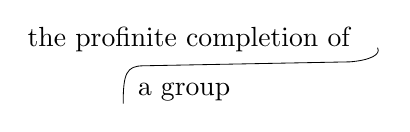
\begin{tikzpicture}[baseline=(base.base)]
\node[anchor=base west,inner sep=0] (base) at (0,0) {a group};
\node[anchor=base west,inner sep=0] at (-1.4,.62) {\inserted{the profinite completion of}};
\draw[line width=.3pt] (-.18,-.10) .. controls (-.18,.28) and (-.14,.38) .. (.08,.38) -- (2.7,.43) .. controls (2.95,.45) and (3.1,.52) .. (3.05,.61);
\end{tikzpicture} of braids $\Pi_{0,\nu}$, which (as an ``outer group'') depends contravariantly on $[1,\nu]$ for monomorphisms.

On $(\mathcal T_{0,\nu})_{\mathbf Q}$ \inserted{of the $(\mathcal T_{\unsure{0\nu|0,\nu}})_{\overline{\mathbf Q}}$} one lets $\mathfrak S_\nu$ act, hence $\mathfrak S_\nu\times\Gamma$ acts on $\mathcal T_{0,\nu}$,
\figure{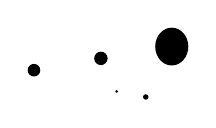
\begin{tikzpicture}[x=1cm,y=1cm]
\fill (0,0) circle (.08);
\fill (.85,.15) circle (.085);
\fill (1.75,.3) ellipse (.21 and .24);
\fill (1.05,-.27) circle (.018);
\fill (1.42,-.34) circle (.035);
\end{tikzpicture}}
\mspage{27}
